\documentclass{standalone}
\usepackage{amssymb,amsmath}
\usepackage{tikz}
\usetikzlibrary{automata,positioning}
\begin{document}
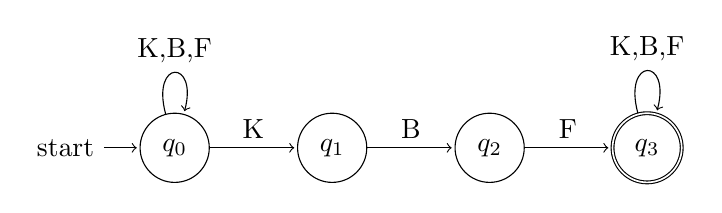
\begin{tikzpicture}[shorten >=1pt,node distance=2cm,on grid,auto] 
 \node[state,initial] (s_0) {$q_0$};
 \node[state] (s_K)[right=of s_0] {$q_1$};
 \node[state] (s_KB)[right=of s_K] {$q_2$};
 \node[state,accepting] (s_KBF)[right=of s_KB] {$q_3$};
 \path[->] 
 (s_0) edge [loop above] node {K,B,F} (s_0)
 (s_0) edge [above] node {K} (s_K)
 (s_K) edge [above] node {B} (s_KB)
 (s_KB) edge [above] node {F} (s_KBF)
 (s_KBF) edge [loop above] node {K,B,F} (s_KBF);
\end{tikzpicture} 
 \end{document}